% METODOLOGIA------------------------------------------------------------------

\chapter{METODOLOGIA}
\label{chap:metodologia}
Com a utilização do \textit{kit} de desenvolvimento STM32F7 \textit{Discovery}, irão ser programadas as tarefas e o \textit{bootloader} que serão os principais componentes desse sistema. As tarefas serão produzidas a partir de bibliotecas já conhecidas e vastamente utilizadas por desenvolvedores de sistemas embarcados, para que assim projetos que necessitem fazer comunicação segura via rede e leitura e escrita de cartões SD, possam utilizar esse sistema de modo a poupar espaço na memória, visando a reutilização dessas bibliotecas, portanto o sistema pode ser amplamente utilizado.
%sistema possa conter intersecções com trechos de codigos utilizados em varios projetos que necessitam

%Adicionar diagrama de blocos!!!!

A partir de um arquivo de \textit{linker}, a memória da plataforma será customizada a fim de abrigar os arquivos necessários para o sistema e protege-los de eventuais sobre-escritas que podem vir a ocorrer. Esse arquivo de \textit{linker}, assim como o \textit{bootloader}, será escrito somente para a plataforma STM32F7, visto que cada plataforma tem suas próprias características como, tamanho de memória e endereços diferentes para cada fabricante e/ou arquitetura. A seguir será explicado parcialmente como funcionarão as funções das tarefas, do \textit{bootloader}, e do servidor HTTP.
%Cada capítulo deve conter uma pequena introdução (tipicamente, um ou dois parágrafos) que deve deixar claro o objetivo e o que será discutido no capítulo, bem como a organização do capítulo.

\section{O \textit{BOOTLOADER}}
\label{sec:Bootloader}

O \textit{bootloader} será responsável em fazer a validação e troca de cada versão de \textit{firmware} instalado no sistema embarcado. Sempre que o sistema for iniciado, o \textit{bootloader} fará a procura de um novo \textit{firmware} na memória interna do sistema. Esse processo, irá verificar o \textit{hash} da nova versão, verificando a integridade e origem do \textit{software}, para então poder ocorrer a atualização. Caso haja alguma falha durante esse processo, o \textit{bootloader} terá a habilidade de verificar esse erro e corrigi-lo, revertendo a atualização, e instalando o \textit{firmware} anterior. O funcionamento do \textit{bootloader} pode ser observado na figura 1.

\begin{figure}[H]
    \scriptsize
     \centering
     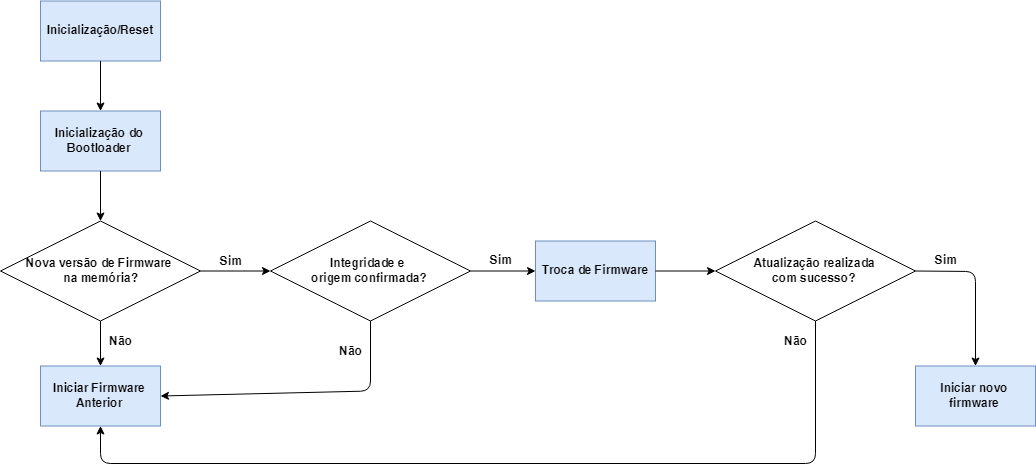
\includegraphics[scale=0.39]{dados/figuras/DiagramaBootloader.png}
     \caption{Diagrama de funcionamento do \textit{bootloader}. Fonte: autoria própria.}
     \label{Diagrama Bootloader}
\end{figure}
%Inserir seu texto aqui...

\section{SERVIDOR HTTP}
\label{sec:ServidorHTTP}

A partir de um computador conectado à mesma rede que o sistema embarcado, haverá um servidor HTTP que ficará responsável por esperar requisições do dispositivo, para consultar a disponibilidade de uma versão atualizada do \textit{software}, e após a confirmação dessa nova versão, esse servidor irá enviar o \textit{firmware} para a plataforma embarcada.
%Inserir seu texto aqui...

\section{TAREFAS DO SISTEMA}
\label{sec:Tarefassistema}

\subsection{COMUNICAÇÃO}

Com o uso da biblioteca LwIP e MbedTLS essa tarefa estará responsável por criar uma comunicação segura entre o \textit{hardware} e o servidor HTTP, a partir dessa comunicação será feito a verificação do sinal de disponibilidade de novo \textit{software} e \textit{download} do mesmo quando o sistema estiver ocioso. 

\subsection{ARMAZENAMENTO}

A partir da utilização da biblioteca FatFs, essa tarefa fará a leitura e escrita sobre um cartão SD instalado no \textit{hardware}. Quando houver a transferência de uma nova versão, tanto o programa anterior quanto o novo, serão colocadas nesta memória, para futuras instalações que serão realizadas pelo \textit{bootloader}. A escolha da mídia de armazenamento de versões do \textit{software} estará a cargo do projetista, sendo escolhido para esse trabalho um cartão SD.


